In this chapter, we outline basics of Ring-$\mathrm{LWE}$ based key-exchange, the idea of reconciliation or key-agreement, basics of existing reconciliation methods and parameter choices to achieve a reasonable security. The goal of this chapter is to examine Ring-$\mathrm{LWE}$ based key-exchange in details and how it aims to be a Diffie-Hellman like replacement candidate.

\section{Key-exchange using \texorpdfstring{$\mathrm{LWE}$}{LWE} and Ring-\texorpdfstring{$\mathrm{LWE}$}{Ring-LWE}}
Basic idea of using $\mathrm{LWE}$ as a key-exchange mechanism is the following: we multiply a randomly generated matrix with a secret, add a noise to it (also known as LWE sample) and then send the randomly generated matrix and $\mathrm{LWE}$ sample to other party.

\begin{figure}[H]
    \centering
% 	$
% 	\begin{bmatrix} 
% 		$Random $  {\mathbb{Z}}^{7 \times 4}_{13} 
% 	\end{bmatrix}
% 	\times
% 	\begin{bmatrix} 
% 		$Secret $  {\mathbb{Z}}^{4 \times 1}_{13} 
% 	\end{bmatrix}
% 	+
% 	\begin{bmatrix} 
% 		$Noise $  {\mathbb{Z}}^{7 \times 1}_{13} 
% 	\end{bmatrix}
% 	=
% 	\begin{bmatrix} 
% 		$Sample result $  {\mathbb{Z}}^{7 \times 1}_{13} 
% 	\end{bmatrix}
% 	$
% 	\vfill
%   
\newcommand{\dimension}{1024}
\newcommand{\error}{16}
\begin{tikzpicture}[scale=0.7]


\node at (-1,2) {\dimension};\draw (0,0) rectangle (4,4);\node at (2,2) {Random};\node at (2,4.5) {\dimension};
\node at (5,2) {$\times$};
\node at (7,4.5) {\error};\draw (6,0) rectangle (8,4);\node at (7,2) {Secret};
\node at (9,2) {$+$};

\node at (11,4.5) {\error};\draw (10,0) rectangle (12,4);\node at (11,2) {Noise};
\node at (13,2) {$=$};
\node at (15,4.5) {\error};\draw (14,0) rectangle (16,4);\node at (15,2) {Sample};

\end{tikzpicture}


	

	\caption{Visualization of $\mathrm{LWE}$ sample}
	$\mathrm{Payload}$: $\text{random } \mathbb{Z}^{\dimension \times \dimension}_{4093}$ and $\text{sample } \mathbb{Z}^{\dimension \times \error}_{4093}$
\end{figure}

Thereafter, other party multiples $\mathrm{LWE}$ sample with his/her secret and result is the shared key. However, matrix multiplication is not commutative, we need to shuffle and transpose key and noise to achieve commutative property. In the following we see the procedure to achieve $16 \times 16$ shared key (i.e. matrix).








\begin{figure}[H]
\centering
\newcommand{\dimension}{1024}
\newcommand{\error}{16}
	\begin{center}
	
\begin{tikzpicture}[scale=0.7]

\node at (-0.65,5) {\dimension};\draw (0,4) rectangle (2,6);\node at (1,5) {$\textbf{A}$};\node at (1,6.5) {\dimension};
\node at (2.5,5) {$\times$};
\node at (3.25,6.5) {\error};\draw (3,4) rectangle (3.5,6);\node at (3.25,5) {$\textbf{s}$};
\node at (3.75,5) {$+$};

\node at (4.25,6.5) {\error};\draw (4,4) rectangle (4.5,6);\node at (4.25,5) {$\textbf{e}$};
\node at (4.75,5) {$=$};
\node at (5.25,6.5) {\error};\draw (5,4) rectangle (5.5,6);\node at (5.25,5) {$\textbf{B}$};

\draw[very thick,->] (6, 3.5) -- (10, 3.5);\draw (7,4) rectangle (7.5,6);\node at (7.25,5) {$\textbf{B}$};\node at (8.9,4.5) {$\in \mathbb{Z}^{\dimension \times \error}_q$};

\node at (10, 5.75) {\error};\draw (10.5,5.5) rectangle (12.5,6);\node at (11.5, 5.75) {$\textbf{s}'$};\node at (11.5, 6.5) {\dimension};
\node at (13, 5) {$\times$};
\node at (14.5, 6.5) {\dimension};\draw (13.5,4) rectangle (15.5,6);\node at (14.5, 5) {$\textbf{A}$};

\node at (16, 5) {$+$};
\draw (16.5,5.5) rectangle (18.5,6);\node at (17.5, 5.75) {$\textbf{e}'$};\node at (17.5, 6.5) {\dimension};
\node at (19, 5) {$=$};
\node at (19.5, 5.75) {\error};\draw (20,5.5) rectangle (22,6);\node at (21, 5.75) {$\textbf{B}'$};\node at (21, 6.5) {\dimension};

\draw[very thick,<-] (6, 0) -- (10, 0);\draw (6.5,1.5) rectangle (8.5,2);\node at (7.5,1.75) {$\textbf{B}'$};\node at (8.5,1) {$\in \mathbb{Z}^{\error \times \dimension}_q$};

\node at (-0.5,1.75) {\error};\draw (0,2) rectangle (2,1.5);\node at (1,2.5) {\dimension};\node at (1,1.75) {$\textbf{B}'$};
\node at (2.5,1) {$\times$};
\node at (3.25,2.5) {\error};\draw (3,0) rectangle (3.5,2);\node at (3.25,1) {$\textbf{s}$};
\node at (4,1) {$=$};
\node at (5,2.5) {\error};\draw (4.5,2) rectangle (5.5,1);\node at (4.10,1.5) {\error};\node at (5,1.5) {$\textbf{K}$};


\node at (10,1.75) {\error};\draw (10.5,1.5) rectangle (12.5,2);\node at (11.5, 1.75) {$\textbf{s}'$};\node at (11.5, 2.5) {\dimension};
\node at (13, 1) {$\times$};
\draw (13.5,0) rectangle (14,2);\node at (3.25,1) {$\textbf{s}$};\node at (13.75,2.5) {\error};\node at (13.75,1) {$\textbf{B}$};
\node at (14.5,1) {$=$};
\node at (15.5,2.5) {\error};\draw (15,2) rectangle (16,1);\node at (14.6,1.5) {\error};\node at (15.5,1.5) {$\textbf{K}$};

\end{tikzpicture}
\end{center}
\caption{Visualization of $\mathrm{LWE}$ based key-exchange}
Resulting shared key is a $\error \times \error$ matrix
\end{figure}


The first issue that emerges is matrix inversion, multiplication are both costly in terms of both space and time. Another important issue is sharing a matrix $\textbf{A}$ is costly with regards to the bandwidth needed for key-exchange. Moreover, to achieve a reasonable security we need at least $1024 \times 1024$ matrix to be shared.

\begin{figure}[H]
\centering
	$\begin{bmatrix} 
		4  & 1  & 11 & 10 \\
		5 & 5 & 9 & 5 \\
		3 & 9 & 8 & 10  \\
		1  & 3 & 3 & 2 
	\end{bmatrix}$
	vs.
    $\underbrace{
    \begin{rcases}
    \begin{bmatrix} 
		2738 & 3842 & 3345 & 2979 & \dots\\
		2896 & 595 & 3607 & \dots \\
		377 & 1575  & \dots \\
        2760 & \dots \\
        \dots
	\end{bmatrix}
    \end{rcases}}_\text{1024 rows}\text{1024 columns}$
	\caption{Toy example $\mathbb{Z}_{13}^{4\times4}$ vs. real-world example $\mathbb{Z}_{4093}^{1024\times1024}$ of random shared matrix}
	{The example on the right is modulo $4093$ so each matrix element in the field of $\mathrm{Z}_{4093}^{1024 \times 1024}$ would require at most $12$ bits. Therefore, $12 \times 1024 \times 1024 = 4291821568 \text{ bits} \approx 1.5 \text{ Megabyte}$}.
\end{figure}

Hence, to overcome above issues we can use cyclic matrices to give matrix some structure and ultimately reduce the size.

\begin{plain}
\normalfont
Circulant matrices (cyclic matrix) form a commutative ring, since for any two given circulant matrices $\textbf{A}$ and $\textbf{B}$, the sum $\textbf{A}+\textbf{B}$ is circulant, the product $\textbf{A} \times \textbf{B}$ is circulant, and $\textbf{A} \times \textbf{B}=\textbf{B} \times \textbf{A}$
\end{plain}

\begin{plain}
\normalfont
A polynomial in a ring $\mathbb{Z}[x] / (x^n-1)$ can be represented as a $n \times n$ circulant matrix. That is:

\[a_0 + a_1x + \dots + a_{n-1}x^{n-1} \mapsto \begin{bmatrix}a_0&a_1 &\dots& a_{n-1} \\a_{n-1}&a_0 &\dots & a_{n-2} \\\dots&\dots&\dots&\dots \\a_{1} & a_2 &\dots& a_0\end{bmatrix}\]
\end{plain}

To solve bandwidth problem, by using cyclic matrix instead then matrix calculation would get a cumulative property for free, so no need to shuffle and transpose matrices as demonstrated previously. As a result, we do not need to send the complete matrix to other party, we can just send the first row and the other party can re-create the matrix. Using polynomials instead of matrix would address the high cost of matrix multiplication and inversion. As noted above, polynomial in $\mathbb{Z}[x] / (x^n - 1)$ can be represented as a cyclic matrix. But as noted before, conjecture is $\mathrm{SVP}_{poly(n)}$ for ideals in $\mathbb{Z}[x]/(f)$ takes time $2^{\Omega(n)}$ when $f$ is irreducible polynomial (if $f$ is not irreducible then multiplication operation would not be invertible in general, and hence we would not get a field and subsequently lattice would not be ideal).


% \begin{figure}[H]
% \centering
% 	$
% 	\begin{bmatrix} 
% 		4  & 1  & 11 & 10 \\
% 		10 & 4  & 1  & 11 \\
% 		11 & 10 & 4  & 1  \\
% 		1  & 11 & 10 & 4  \\
% 		4  & 1  & 11 & 10
% 	\end{bmatrix}
% 	\to
% 	\begin{bmatrix} 
%         4  & 1  & 11 & 10 \\
% 	    3  & 4  & 1  & 11 \\
% 	    2  & 3  & 4  & 1  \\
% 	    12 & 2  & 3  & 4  \\
% 	    9  & 12 & 2  & 3  \\
% 	    10 & 9  & 12 & 2  \\
% 	    11 & 10 & 9  & 12 \\
% 	    1  & 11 & 10 & 9  \\
% 	    4  & 1  & 11 & 10
% 	\end{bmatrix}$
% 	\caption{Demonstration of cyclic matrix in $\mathrm{LWE}$ (toy example)}
% 	\footnotesize{Note that we do not need to sent the complete matrix, sending the first row is enough to re-create the matrix.	Also, after first $4$ rows on the left and $2 \times 4 = 8$ rows on the right, rows are repeating so no new vector is introduced after those rows.}
% \end{figure}

Simple irreducible polynomial can be: $x^n + 1$. We can use a wrapping rule to represent a polynomial in $\mathbb{Z}[x] / (x^n + 1)$ when $n$ is a power of $2$. This would remove any pattern in cyclic matrix and subsequently makes it more complex. The wrapping rule can be: ${x \mapsto -x \bmod \ 13}$ applied to the shifted value. In other words, do a circular right shift to every row and apply above map to the value of first column of shifted row.


Below shows that by treating the first row of cyclic matrix as a polynomial in quotient polynomial ring over finite field of $\mathbb{Z}_{13}[x] / ( x^{4} + 1 )$, polynomial can be represented as a wrapping rule described above (i.e. $\mathbb{Z}^{4 \times 4}_{13}$). In details, we can construct the same matrix using the first row of matrix as a polynomial in quotient ring over finite field and then multiplying it by $x^i$ for $0 \le i < n$ to re-create original matrix.


\begin{figure}[H]
\centering
    $\begin{bmatrix} 
            4& 1& 11& 10\\
    	    3& 4& 1& 11\\
    	    2& 3& 4& 1\\
    	    12& 2& 3& 4
    \end{bmatrix}
    \leftrightarrow
    \begin{matrix} 
            x^0 \times (4x^0+ 1x^1+ 11x^2+ 10x^3) = 4x^0+ 1x^1+ 11x^2+ 10x^3 \to [4, 1, 11, 10]\\
    	    x^1 \times (4x^0+ 1x^1+ 11x^2+ 10x^3) = 3x^0+ 4x^1+ 1x^2+ 11x^3  \to [3, 4, 1, 11]\\
    	    x^2 \times (4x^0+ 1x^1+ 11x^2+ 10x^3) = 2x^0+ 3x^1+ 4x^2+ 1x^3 \to [2, 3, 4, 1]\\
    	    x^3 \times (4x^0+ 1x^1+ 11x^2+ 10x^3) = 12x^0+ 2x^1+ 3x^2+ 4x^3 \to [12, 2, 3, 4]\\
     \end{matrix}$
     \caption{Demonstration of simple wrapping rule to create cyclic matrix in Ring-$\mathrm{LWE}$}
     It is essentially multiplying the first row with $x^i$ for $i \in [0, n-1]$ and extract coefficients.
\end{figure}



The above wrapping rules helps to visualize Ring variant of LWE where irreducible polynomial is $x^n + 1$, in terms of a matrix. But polynomial multiplication is substantially more efficient in terms of both space and time. So by using Ring variant of LWE (i.e. treating $A, s, e$ as polynomials instead of matrices), we can make key-exchange process substantially more efficient. 


\iftoggle{verylong}{
\lstinputlisting[language=Python, caption=Implementation of wrapping rule and testing if it equals to Quotient ring in SageMath]{code_snippets/cyclic_matrix_rlwe.sage}
}{}



\subsection{Reason to use a reconciliation method}
Below is a Diffie-Hellman like key-exchange in Ring-$\mathrm{LWE}$. Note that $A$ is a shared polynomial, $s$ is a secret polynomial and $e$ is a noise polynomial. Only polynomials $A$ and $b$ are shared between two parties and $s, e$ are both kept secret. 

\begin{figure}[H]
    \centering
	Alice chooses {small} $s$, $e$ in ${\mathbb{Z}}_{q}$, both sampled from a noise distribution\\
	Bob chooses {small} $s'$, $e'$ in ${\mathbb{Z}}_{q}$, both sampled from a noise distribution\\
	Alice $\to$ Bob: $b = A \times s + e$\\
	Bob $\to$ Alice: $b' = A \times s' + e'$\\
	Shared secret Alice calculates: $s \times b' = s \times (A \times s' + e') = A \times s   \times s' + \boldsymbol{s \times e'}$\\
	Shared secret Bob calculates: $s' \times b = s' \times (A \times s + e) = A \times s   \times s' + \boldsymbol{s' \times e}$
	\caption{Basic Ring-$\mathrm{LWE\text{-}DH}$ key agreement}
	{$A$ is similar to generator ($g$) and $q$ (prime) is similar to modulo prime in Diffie-Hellman key exchange}
\end{figure}

Notice that shared keys do not match because ${s} \times {e}' \neq {s}' \times {e}$. Although errors are supposed be relatively small compared to shared polynomial ${A}$ and their product with secret would be small as a result (i.e. $||{s} \times {e}'|| , ||{s}' \times {e}|| \ll ||A||$), but still resulting shared key do not match and it is a problem if one wants to construct a cryptographic key-exchange protocol. To overcome this issue we use rounding methods to extract a bit from every coefficient and as added error is relatively small, hence, the coefficients would not differ significantly. Therefore, rounding method eliminates the error and extracts the same shared key for both parties. There are two types of rounding methods (or reconciliation techniques): 

\begin{enumerate}
    \item reconciliation without any rounding information (e.g. Regev's basic rounding method)
    \item reconciliation with rounding information to substantially increase the probability of extracting the same key.
\end{enumerate}

The idea of sending extra bits was initially introduced by Ding and later improved by Peikert and Alkim et al.

\begin{lemma}
    \normalfont
    (\cite{DBLP:conf/crypto/ApplebaumCPS09}, Lemma 2)
    $\mathrm{LWE}$ is no easier if the secret is drawn from the error distribution $\chi^{n}$
    % This is also called the \text{Hermite normal form} of $\mathrm{LWE}$ \cite{Micciancio2009}.
\end{lemma}

The advantage to sample $\textbf{s}$ and $\textbf{e}$ from normal distribution (Gaussian) is the guarantee that $\langle \textbf{s}, \textbf{e} \rangle$ is small. Hence, during decryption, terms that look like $\langle \textbf{s}, \textbf{e} \rangle$ (inner product of the secret vector $\textbf{s}$ and error vector $\textbf{e}$) appears in the decryption. In Ring variant of key-exchange, we receive as shared key ${s} \times ({A} {s}'+{e}')={A} {s}{s}'+{s}{e}' \leftrightarrow {s}' \times ({A} {s}+{e})={A} {s} {s}'+{s}' {e}$. So if both parties choose small $s$ and $s'$ (hence their inner product with error terms would be small) and then chance of reconciliation failing to extract the same key would be reduced substantially. 


% \begin{plain}
%     \normalfont
% There is an advantage to sample $s$ and $e$ from normal distribution (Gaussian):
% \begin{itemize}
%     % \item Guarantees that $\textbf{s}$ and $\textbf{e}$ have large norms (Euclidean norm)
%     \item Guarantees that $\langle s, e \rangle$ is small
%     \item Gaussian distribution has relatively high entropy in comparison with uniform distribution (discrete uniform sampler from $[0,  \sigma)$) and achieves the above properties
% \end{itemize}
% \end{plain}

% \begin{definition}
% \normalfont
% Given a basis $\textbf{B} =\{\mathbf{b} _{1},\mathbf {b} _{2},\dots ,\mathbf {b}_{d}\}$ with $n$-dimensional integer coordinates, for a lattice $\mathcal{L}$ (a discrete subgroup of $\mathbb{R}^n$) with $d\leq n$, the $\mathrm{LLL}$ algorithm calculates an $\mathrm{LLL}$-reduced (short, nearly orthogonal) lattice basis in time $\mathcal{O}(d^{5}n\log ^{3}B)$, where .
% \end{definition}

% The $l_{2}$ norm is important in cryptanalysis. When an attacker is trying to recover the secret key or the message, he will set up a lattice and try to find a short vector. We know how to judge the running time of lattice-reduction algorithms based on the $l_{2}$ norm of the vector they are trying to find. In particular, $\mathrm{LLL}$ (and its variants) are analyzed in terms of the $l_{2}$ norm (i.e. time complexity of $\mathrm{LLL}$ is $\mathcal{O}(d^{5}n\log ^{3}B)$ where $B$ is the largest length of $b_{i}$ under the Euclidean norm $l_{2}$).


\section{Reconciliation methods}
Below is a description of different reconciliation methods in Ring-$\mathrm{LWE}$. These methods apply to every coefficient of resulting shared key which is a polynomial in Ring-$\mathrm{LWE}$. These methods can also be applied to $\mathrm{LWE}$ based key-exchange as well by applying them to respective matrix elements.


\subsection{Rounding method in Ring-\texorpdfstring{$\mathrm{LWE}$}{LWE} suggested by Regev}
As each coefficient of polynomial is an integer modulo $q$, then we can round each coefficient to either to $0$ or $1$. Regev's suggested to round every coefficient if it in $( \frac{-q}{2}, \frac{-q}{4}] \cup (\frac{q}{4}, \frac{q}{2}]$ to $1$, and round if it is in $(\frac{-q}{ 4}, \frac{q}{4}]$ to $0$. This basic method works most of the time and probability of failure is $\frac{1}{2^{10}}$ which is not good enough considering that we have $1024$ coefficients in our shared polynomial to achieve a reasonable security.



\begin{figure}[H]
	\centering
	\begin{tabular}{|lll|}
		\hline
		\textbf{Alice}                                       &                               & \textbf{Bob}                               \\\hline
		$s, e \gets \chi$, $A \gets \text{uniformly random}$ &                               & $s', e' \gets  \chi$                       \\
		                                                     & $\xrightarrow{ A, b = As + e}$ &                                            \\
		                                                     & $\xleftarrow{b' = As' + e'}$  &                                            \\
				 		
		$K = \texttt{reconcile}(s \times b')$          &                               & $K = \texttt{reconcile}(s' \times b)$ \\\hline
	\end{tabular}
	\caption{Diagram of basic Diffie-Hellman like key-exchange protocol in Ring-$\mathrm{LWE}$}
    \figuresubtitle{Note that $s, e$ and $s', e'$ are all sampled from a noise distribution but $A$ is generated uniformly at random. Also, \texttt{reconcile} function applies Regev's basic rounding method to every coefficient of resulting polynomial.}
\end{figure}

\begin{figure}[H]
	\begin{center}
		\begin{tikzpicture}
			\draw (2,2) circle (1cm);
			\draw (2,2) -- (2,3);
			\draw (2,2) -- (2,1);
											
			\node at (3.5,2) {$0$};
			\node at (2,3.5) {$\frac{q}{4}$};
			\node at (0.5,2) {$\frac{q}{2}$};
			\node at (2,0.5) {$\frac{3q}{4}$};
											
			\node at (2.5,2) {$\mapsto 0$};
			\node at (1.5,2) {$\mapsto 1$};
											
		\end{tikzpicture}
	
	Alice's calculated shared key:
	    
	$4079331x^0 + 1894732x^1 + \dots + 472608x^{1022} + 516748x^{1023} = 01 \dots 00$
	\\~\\ 
	Bob's calculated shared key:
	    
	$4079332x^0 + 1894733x^1 + \dots + 472607x^{1022} + 516748x^{1023} = 01 \dots 00$
	\caption{Demonstration of Regev's rounding approach}
	\figuresubtitle{Notice coefficients of both parties are close but not equal. In Regev's rounding approach, we round each efficient to either $0$ or $1$ based on the region coefficient is located at.}
    \end{center}
\end{figure}



\subsection{Improved rounding method as suggested by Ding}
Regev's method can be modified slightly by multiplying error terms by $2$. The goal is to make sure difference between error terms would be even. Thereafter, we would follow the naive approach of $\bmod 2$ to eliminate the terms $2 \times s \times e'$ and $2 \times s' \times e$, hence, resulting shared key would match. However this would not result in any improvement because difference between calculated key of both parties would not always be even, since we are working in $\mathbb{Z}_{q}$ as oppose to $\mathbb{Z}$ and $q$ is an odd prime. Therefore, further adjustments are needed.


\begin{figure}[H]
    \centering
	Alice chooses {small} $s$, $e$ in ${\mathbb{Z}}_{q}$, both sampled from a noise distribution\\
	Bob chooses {small} $s'$, $e'$ in ${\mathbb{Z}}_{q}$, both sampled from a noise distribution\\
	Alice $\to$ Bob: $b = A \times s + 2 \times e$\\
	Bob $\to$ Alice: $b' = A \times s' + 2 \times e'$\\
	Shared secret Alice calculates: $s \times b' = s \times (A \times s' + 2 \times e') = A \times s   \times s' + 2\times s \times e'$\\
	Shared secret Bob calculates: $s' \times b = s' \times (A \times s + 2 \times e) = A \times s   \times s' + 2 \times s' \times e$
	$A \times s   \times s' + 2\times s \times e' - A \times s   \times s' + 2 \times s' \times e = 2 \times (s\times e' - s' \times e)\leftarrow \textbf{not necessarily even difference}$
	\caption{Demonstration of using even error values in basic Ring-$\mathrm{LWE\text{-}DH}$ key agreement}
	\figuresubtitle{For example, in $\mathbb{Z}$, $2 \times 7 = 14$ which is an even number but in $\mathbb{Z}_{13}$, it would be $1$ which is an odd number.}
\end{figure}


\begin{figure}[H]
    \centering
	\begin{center}
    \begin{tikzpicture}[scale=0.95]
			\draw (2,2) circle (1cm);
			\draw (2,2) -- (2,3);
			\draw (2,2) -- (2,1);
											
			\node at (3.5,2) {$0$};
			\node at (2,3.5) {$\frac{q}{4}$};
			\node at (0.5,2) {$\frac{q}{2}$};
			\node at (2,0.5) {$\frac{3q}{4}$};
											
			\node at (2.5,2) {$\mapsto 0$};
			\node at (1.5,2) {$\mapsto 1$};

    		\fill (2.3,2.95)  circle[radius=2pt];
    		\fill (1.7,2.95)  circle[radius=2pt];
		
            \draw[-stealth] (-3,-1)--(6,-1);
            \node at (7, -1){x};
            \node at (7, 0) {$\mathbb{Z}$};
            \draw (-2, -1)  circle[radius=2pt];\node at (-2, -1.5) {-2};			
            \draw (-1, -1)  circle[radius=2pt];\node at (-1, -1.5) {-1};
            \draw (0, -1)  circle[radius=2pt];\node at (0, -1.5) {0};
            \draw (1, -1)  circle[radius=2pt];\node at (1, -1.5) {1};
            \draw (2, -1)  circle[radius=2pt];\node at (2, -1.5) {2};
            \draw (3, -1)  circle[radius=2pt];\node at (3, -1.5) {3};
            \draw (4, -1)  circle[radius=2pt];\node at (4, -1.5) {4};
            \draw (5, -1)  circle[radius=2pt];\node at (5, -1.5) {5};
            
            \fill (2,-1)  circle[radius=4pt];
            \fill (4,-1)  circle[radius=4pt];
            \draw[thick,|<->|] (2, -0.5) -- (4, -0.5); 	
            \draw (2, -1) -- (2, 0); 	
            \draw (4, -1) -- (4, 0); 
            
            \draw[-stealth] (-3,-4)--(6,-4);
            \node at (7, -4){x};
            \node at (7,-3) {$\mathbb{Z}_{q}$ (e.g. $\mathbb{Z}_{5} \in \{-2, -1, 0, 1, 2\}$)};
            \draw (-2, -4)  circle[radius=2pt];\node at (-2, -4.5) {-2};			
            \draw (-1, -4)  circle[radius=2pt];\node at (-1, -4.5) {-1};
            \draw (0, -4)  circle[radius=2pt];\node at (0, -4.5) {0};
            \draw (1, -4)  circle[radius=2pt];\node at (1, -4.5) {1};
            \draw (2, -4)  circle[radius=2pt];\node at (2, -4.5) {2};
            \draw (3, -4)  circle[radius=2pt];\node at (3, -4.5) {3};
            \draw (4, -4)  circle[radius=2pt];\node at (4, -4.5) {4};
            \draw (5, -4)  circle[radius=2pt];\node at (5, -4.5) {5};
            
            \fill (2,-4)  circle[radius=4pt];
            \fill (-1,-4)  circle[radius=4pt];
            \draw[thick,|<->|] (2, -3.5) -- (-1, -3.5); 	
            \draw (2, -4) -- (2, -3); 	
            \draw (-1, -4) -- (-1, -3); 
		\end{tikzpicture}
		\end{center}
		\caption{Demonstration of only multiplying errors by $2$ will not help the reconciliation}
		\figuresubtitle{In $\mathbb{Z}$ difference between two points is even but in $\mathbb{Z}_{5}$ difference is odd, hence no benefit in just multiplying error terms by $2$. More than just multiplying error terms by $2$ is needed.}
\end{figure}




Ding in \cite{ding2012simple} proposed a reconciliation method based on Ring-$\mathrm{LWE}$. This protocol is the first to introduce the idea of sending extra information to improve success rate of reconciliation. Peikert improved Ding's method in \cite{peikert2014lattice} and presented a $\mathrm{KEM}$ (key-exchange mechanism). Later on Peikert's $\mathrm{KEM}$ was used in the construction of the $\mathrm{BCNS}$ protocol \cite{bos2015post} which itself was recently improved, resulting in the $\mathrm{NewHope}$ protocol by Alkim et al. \cite{alkim2015post}.

The basic idea of Ding's method can be seen as Diffie-Hellman like key exchange protocol based on the Ring-$\mathrm{LWE}$ problem. The key-exchange protocol is secure against passive adversaries if Ring-$\mathrm{LWE}$ is hard. For a proof and an exact definition of this security model we refer to \cite{ding2012simple}. The key exchange protocol is only proven to be secure in the two-user setting. A multi-user variant is proposed in the same paper, but its security is not yet proven. To describe Ding's reconciliation method, we define the following functions: $\delta: \mathbb{Z}_{q} \mapsto \{0, 1\}$, $Signal: \mathbb{Z}_{q} \mapsto \{0, 1\}$, and $Encode: \mathbb{Z}_{q} \times \{0, 1\} \mapsto \{0, 1\}$ via:

\begin{equation}
Signal(x) = \delta(x) \mapsto
\begin{cases*}
  0 & if $x \in [-\lfloor \frac{q}{4} \rfloor$, $\lfloor\frac{q}{4} \rceil]$\\
  1 & otherwise
\end{cases*}
\end{equation}

% \begin{equation}
% \delta_{1}(x) =
% \begin{cases*}
%   0 & if $x \in [-\lfloor \frac{q}{4}\rfloor +1$, $\lfloor\frac{q}{4}\rfloor +1]$\\
%   1 & otherwise
% \end{cases*}
% \end{equation}

% \begin{equation}
% Signal(x) = \delta(x)
% \end{equation}

\begin{equation}
Encode(x, \delta) = (x + \delta \times (\frac{q-1}{2}) \bmod q) (\bmod 2)
\end{equation}





The basis idea is that if coefficient is in inner region ($\delta = 0$) , then we just $\bmod 2$ because the difference between $2 \times s \times e'$ and $2 \times s'\times e$ is even with high probability, hence in inner region the probability of achieving the same $\bmod 2$ of coefficient is much higher than outer region. What we want to avoid while $\bmod 2$ is coefficient of two parties are in different regions. So, if signal bit is in outer region ($\delta = 1$), then we add $\frac{q-1}{2}$ to respective coefficient. Therefore, coefficient will now be in inner region and then $\bmod 2$.



\begin{figure}[H]
    \centering
	\begin{center}
    \begin{tikzpicture}
			\draw (2,2.1) circle (1cm);
			\draw (2,2.1) -- (2,3.1);
			\draw (2,2.1) -- (2,1.1);
											
			\node at (3.5,2.1) {$0$};
			\node at (2,3.6) {$\frac{q}{4}$};
			\node at (0.5,2.1) {$\frac{q}{2}$};
			\node at (2,0.8) {$\frac{3q}{4}$ or $\frac{-q}{4}$};
											
			\node at (2.5,2.1) {$\mapsto 0$};
			\node at (1.5,2.1) {$\mapsto 1$};


            \draw[-stealth] (-3,-1)--(6.5,-1);
            \node at (7, -1){x};
            \node at (7, 0) {$\mathbb{Z}_{q}$};
            \draw (-2, -1)  circle[radius=2pt];\node at (-2, -1.5) {$\frac{-(q-1)}{2}$};			
            \draw (0, -1)  circle[radius=2pt];\node at (0, -1.5) {$\frac{-q}{4}$};			
            \draw (2, -1)  circle[radius=2pt];\node at (2, -1.5) {$0$};	
            \draw (4, -1)  circle[radius=2pt];\node at (4, -1.5) {$\frac{q}{4}$};			
            \draw (6, -1)  circle[radius=2pt];\node at (6, -1.5) {$\frac{(q-1)}{2}$};			

            \fill (6,-1)  circle[radius=4pt];
            \fill (4,-1)  circle[radius=4pt];
            \draw[thick,|<->|] (4, -0.5) -- (6, -0.5); 	
            \draw (4, -1) -- (4, 0); 	
            \draw (6, -1) -- (6, 0); 
  			\node at (5,0.3) {outer: $\delta = 1$};

            \fill (-2,-1)  circle[radius=4pt];
            \fill (0,-1)  circle[radius=4pt];
            \draw[thick,|<->|] (-2, -0.5) -- (0, -0.5); 	
            \draw (-2, -1) -- (-2, 0); 	
            \draw (0, -1) -- (0, 0); 
  			\node at (2,0) {inner: $\delta = 0$};

            \fill (0,-1)  circle[radius=4pt];
            \fill (4,-1)  circle[radius=4pt];
            \draw[thick,|<->|] (0, -0.5) -- (4, -0.5); 	
            \draw (4, -1) -- (4, 0); 	
            \draw (6, -1) -- (6, 0); 
  			\node at (-1,0.3) {outer: $\delta = 1$};

    		\draw[very thick,<-] (-1,-1.5) -- (0,-3);
    		\draw[very thick,<-] (3,-1.5) -- (0,-3);
    		\node at (0, -3.5){add $\frac{(q-1)}{2}$};
    
    		\draw[very thick,<-] (1,-1.5) -- (4,-3);
    		\draw[very thick,<-] (5,-1.5) -- (4,-3);
            \node at (4, -3.5){add $\frac{(q-1)}{2}$};
    

		\end{tikzpicture}
		\end{center}
		\caption{Demonstration of signal function in $\mathrm{DXL}$ protocol}
		\figuresubtitle{If $\delta = 1$ or we are in outer region, then we add $\frac{q-1}{2}$ to respective coefficient, hence we will be in inner region and then $\bmod 2$; if $\delta = 0$ then we just $\bmod 2$.}
\end{figure}



% \subsection*{\texorpdfstring{$\mathrm{DXL}$}{DXL} Protocol construction}
Ding in the same paper introduced $\mathrm{DXL}$ key-exchange protocol. However, this protocol never got implemented in an efficient manner but it had an impact on future key-exchange protocols. For example, adding secondary noise to the calculated polynomial key to prevent secret leakage and increase entropy (additive noise).

The key exchange in this protocol will take place between two parties. There will be an initiator for the key exchange designated as ($I$) and a respondent designated as ($R$). Both $I$ and $R$ know $q$, $n$, $a(x)$, and have the ability to generate small polynomials according to the distribution $\chi_{\sigma}$ with parameter $\sigma$. The distribution $\chi_{\sigma}$ is a discrete Gaussian distribution. The key-exchange begins with the initiator ($I$) doing the following:

\noindent\textbf{Initiation}
\begin{enumerate}
    \item Generate two polynomials $s_{I}$ and $e_{I}$ with small coefficients by sampling from the distribution $\chi _{\sigma }$.
    \item Compute $p_{I}=as_{I}+2e_{I}$.
    \item The initiator sends the polynomial $p_{I}$ to the Responder.
\end{enumerate}

\noindent\textbf{Response}
\begin{enumerate}
    \item Generate two polynomials $s_{R}$ and $e_{R}$ with small coefficients by sampling from the distribution $\chi _{\sigma }$
    \item Compute $p_{R}=as_{R}+2e_{R}$
    \item Generate a small $e'_{R}$ from $\chi _{\sigma }$. Compute $k_{R}=p_{I}s_{R}+2e'_{R}$. Then $k_{R}=as_{I}s_{R}+2e_{I}s_{R}+2e'_{R}$
    \item Use the signal function $Signal$ to find $w=Signal(k_{R})$. This is computed by applying $Signal$ function on each coefficient of $k_{R}$
    \item Respondent side's key stream $sk_{R}=Encode(k_{R}, w)$ is calculated, based on the reconciliation information $w$ and the polynomial $k_{R}$
    \item The Respondent sends $p_{R}$ and $w$ to the Initiator
\end{enumerate}

\noindent\textbf{Finish}
\begin{enumerate}
    \item Receive $p_{R}$ and $w$ from the Responder
    \item Sample $e'_{I}$ from $\chi _{\sigma }$ and Compute $k_{I}=p_{R}s_{I}+2e'_{I}=as_{I}s_{R}+2e_{R}s_{I}+2e'_{I}$
    \setcounter{enumi}{0}
    \item Initiator side's key stream is produced as $sk_{I}=Encode(k_{I}, w)$ from the reconciliation information $w$ and polynomial $k_I$
\end{enumerate}









\subsection{Rounding method as utilized in $\mathrm{BCNS}$ protocol}
In 2014, Peikert in \cite{peikert2014lattice} presented a key transport scheme following the same basic idea of Ding's, where the idea of sending additional $1$ bit signal for every coefficient is also utilized. In this improved approach, Bob sends Alice a reconciliation information $\in \{0,1\}^n$ (similar to output of signal function in Ding's method) such that $0 \mapsto region\ \#1$, $1 \mapsto region\ \#2$. In other words, as a reconciliation information one party sends a region number that his or her coefficient is located in. Then based on the region, a particular key extraction rule applies. If $v, u$ are respective coefficients of Alice and Bob, and also $|u-v| \le \frac{q}{8}$, then this method always works. Due to the clever design of rounding regions and key extractions rules, revealing the region leaks no information and does not compromises security.

We should note that $\mathrm{BCNS}$ protocol is an implementation of Peikert's reconciliation method and this protocol does not introduce a new reconciliation method.

\begin{figure}[H]
	\centering
	\begin{subfigure}[t]{0.3\textwidth}
		\centering
		\begin{tikzpicture}
			\draw (2,2) circle (1cm);
			\draw (2,2) -- (2,3);
			\draw (2,2) -- (2,1);
			\draw (2,2) -- (3,2);
			\draw (2,2) -- (1,2);
											
			\node at (3.5,2) {$0$};
			\node at (2,3.5) {$\frac{q}{4}$};
			\node at (0.5,2) {$\frac{q}{2}$};
			\node at (2,0.5) {$\frac{3q}{4}$};
													
			\node at (2.5,2.35) {\#1};
			\node at (2.5,1.65) {\#2};
									
			\node at (1.5,2.35) {\#2};
			\node at (1.5,1.65) {\#1};
		\end{tikzpicture}
		\caption{4 rounding regions}
	\end{subfigure}
	\hfill
	\begin{subfigure}[t]{0.3\textwidth}
		\centering
		\begin{tikzpicture}
			\draw (2,2) circle (1cm);
			\draw (2,2) -- (1.3,2.7);
			\draw (2,2) -- (2.7,1.3);
						
			\node at (3.5,2) {$0$};
			\node at (2,3.5) {$\frac{q}{4}$};
			\node at (0.5,2) {$\frac{q}{2}$};
			\node at (2,0.5) {$\frac{3q}{4}$};
									
			\node at (2.5,2) {$\mapsto 0$};
			\node at (1.5,2) {$\mapsto 1$};
		\end{tikzpicture}
		\caption{Case \#1}
	\end{subfigure}    
	\hfill
	\begin{subfigure}[t]{0.3\textwidth}
		\centering
		\begin{tikzpicture}
			\draw (2,2) circle (1cm);
			\draw (2,2) -- (2.7,2.7);
			\draw (2,2) -- (1.3,1.3);
						
			\node at (3.5,2) {$0$};
			\node at (2,3.5) {$\frac{q}{4}$};
			\node at (0.5,2) {$\frac{q}{2}$};
			\node at (2,0.5) {$\frac{3q}{4}$};
									
			\node at (2.5,2) {$\mapsto 0$};
			\node at (1.5,2) {$\mapsto 1$};
		\end{tikzpicture}
		\caption{Case \#2}
	\end{subfigure}
	\caption{Demonstration of Peikert's rounding approach}
	\figuresubtitle{(a) demonstrates the $4$ regions and (b) is a rounding rule when
	rounding information bit indicates regions \#1 and (c) if it indicates region \#2. Notice if difference of coefficients is $\le \frac{q}{8}$ then this method always works.}
\end{figure}		

% To improve polynomial multiplication speed, we can use $\mathrm{FFT}$ such that rather than working modulo degree-$1024$ polynomial with coefficients in ${\mathbb{Z}}_{q}$, we can work with degree-$256$ polynomial whose coefficients are themselves polynomials modulo a degree-$4$ polynomial. 
 

\begin{figure}[H]
    \centering
	Alice chooses \textit{small} $s$, $e$ in ${\mathbb{Z}}_{q}$, both sampled from a noise distribution\\
	Bob chooses \textit{small} $s'$, $e'$ in ${\mathbb{Z}}_{q}$, both sampled from a noise distribution\\
	Alice $\to$ Bob: $b = A \times s + e$\\
	Bob $\to$ Alice: $b' = A \times s' + e'$ and \textbf{rounding region} $ \in \{0,1\}^{n}$\\
	Shared secret Alice calculates: $s \times b' = s \times (A \times s' + e') = s \times A \times s' + s \times e'$\\
	Shared secret Bob calculates: $s' \times b = s' \times (A \times s + e) = s' \times A \times s + s' \times e$
	\caption{Exact Ring-$\mathrm{LWE\text{-}DH}$ key agreement as suggested by Peikert.}
	\figuresubtitle{Notice Bob also sends his rounding regions to Alice which is similar to Ding's rounding method}
\end{figure}		
		
% \subsubsection{\texorpdfstring{$\mathrm{KEM}$}{KEM} protocol description as suggested by Peikert}	

The following is the concrete description of Peikert's reconciliation method. We define the reconciliation mechanism where the modulus $q \ge 2$ is even, then define disjoint intervals $I_{0} = \{0, 1, \dots, \lfloor \frac{q}{4} \rceil- 1\}$, $I_{1} =  \{\lfloor \frac{3q}{4}\rceil, \dots, q-1\} \bmod q$. Now define the \textit{cross-rounding} function $\langle \cdot \rangle _{2}: \mathbb{Z}_{q} \to \mathbb{Z}_{2}$ as:


% $\langle v \rangle _{2}: = \lfloor \frac{4}{q} \cdot v \rfloor \bmod 2$. Equivalently, $\langle v \rangle_{2}$ is the $b \in \{0, 1\}$ such that $v$ belongs to the disjoint union $I_{b} \cup (\frac{q}{2} + I_{b})$.
 
% We see that these intervals form a partition of all the elements $v \in \mathbb{Z}_{q}$ such that $\lfloor v \rceil _{2} = 0$ (where we identify $0$ and $1$ with their residue classes modulo two). Similarly, $\frac{q}{2} + I_{0}$ and $\frac{q}{2} + I_{1}$ partition all the $v$ such that $\lfloor v \rceil _{2} = 1$.


% Let $q$ be an even modulus. Then we obtain:
% \[
% \lfloor v \rceil_{q, 2}  
% \begin{cases}
%     1 & v \in \{\lfloor \frac{q}{4} \rceil, \dots, \lfloor \frac{3q}{4} \rceil - 1 \} \\
%     0 &  v \in \{ 0, 1, \dots, \lfloor \frac{q}{4} \rceil - 1\} \cup \{ \lfloor \frac{3q}{4} \rceil, \dots, q - 1\}
% \end{cases}
% \]

% If $v$ is uniformly random, then $\langle v \rangle _{2}$ is uniformly random if and only if $\frac{q}{2}$ is even; otherwise, $\langle v \rangle_{2}$ is biased toward zero. Regardless of this potential bias, however, the theorem below shows that $\langle v \rangle_{2}$ hides $\lfloor v \rceil _{2}$ perfectly. 

% \begin{theorem}
%     \normalfont
%     For even $q$, if $v \in \mathbb{Z}_{q}$ is uniformly random, then $\lfloor v \rceil _{2}$ is uniformly random given $\langle v \rangle_{2}$.
% \end{theorem}

% \begin{theorem}
%     \normalfont
%     For even $q$, if $w = v + e \bmod q$ for some $v \in \mathbb{Z}_{q}$ and $e \in E$, then $\mathrm{rec}(w,\langle v \rangle_{2}) = \lfloor v \rceil _{2}$
% \end{theorem}

% The following is cross-rounding function:

\[
\langle v \rangle_{q, 2}=  
\begin{cases}
    0 & v \in I_{0} \cup (I_{0} + \frac{q}{2}) \\
    1 & v \in I_{1} \cup (I_{1} + \frac{q}{2})
\end{cases}
\]

% Let $I'_{1} = \{ \lfloor \frac{q}{2} \rfloor, \dots, -1\}$ and $I'_{0} = \{ 0, 1, \dots, \lfloor \frac{q}{2} \rceil -1 \}$. 

To compute the shared key the following reconciliation function $\text{rec}: \mathbb{Z}_{q} \times \mathbb{Z}_{2} \to \mathbb{Z}_{2}$ is used:

\[
\text{rec}(v, b) =
\begin{cases}
    0 & \text{if } v \in I_{b} + ([-\frac{q}{8}, \frac{q}{8}) \cap \mathbb{Z}) \bmod q\\
    % [-\frac{q}{2}, \frac{q}{2}) \\
    1 & \text{otherwise}
\end{cases}
\]


All of the above applies when $q$ is even, but in applications of Ring-$\mathrm{LWE}$ this is not the case. For instance, it is often desirable to let $q$ be a sufficiently large prime, for efficiency and security reasons. When $q$ is odd, while it is possible to use the above methods to agree on a bit derived by rounding a uniform $v \in \mathbb{Z}_{q}$, the bit will be biased, and hence not suitable as key material. Here we show how to avoid such bias by temporarily \textit{scaling up} to work modulo $2q$, and introducing a small amount of extra randomness.

Define the randomized function $\mathrm{dbl}: \mathbb{Z}_{q} \to \mathbb{Z}_{2q}$ that, given a $v \in \mathbb{Z}_{q}$, outputs $\bar{v} = 2v - \bar{e} \in \mathbb{Z}_{2q}$ for some random $\bar{e} \in \mathbb{Z}$ that is uniformly random modulo two and independent of $v$, and small in magnitude (e.g., bounded by one).


\[
\text{dbl}: \mathbb{Z}_q \to \mathbb{Z}_{2q}, x\mapsto2x - \bar{e}, \text{ where } \bar{e} = 
\begin{cases}
    -1 & \text{with probability } \frac{1}{4}\\
    0 & \text{with probability } \frac{1}{2}\\
    1 & \text{with probability } \frac{1}{4}\\
\end{cases}
\]


Moreover, if $w, v \in \mathbb{Z}_{q}$ are close, then so are $2w, \mathrm{dbl}(v) \in \mathbb{Z}_{2q}$, i.e., if $w = v+e (\bmod q)$ for some (small) $e$, thus $2e$ would be small too, then $2w = \bar{v} + (2e + \bar{e}) (\bmod 2q)$. Therefore, to (cross-) round from $\mathbb{Z}_{q}$ to $\mathbb{Z}_{2}$, we simply apply $\mathrm{dbl}$ to the argument and then apply the appropriate rounding function from $\mathbb{Z}_{2q}$ to $\mathbb{Z}_{2}$. Similarly, to reconcile some $w \in \mathbb{Z}_{q}$ we apply rec to $2w \in \mathbb{Z}_{2q}$; note that this process is still deterministic.

To summarize, The usual definition of (passive) security for key-exchange requires the agreed-upon key to be indistinguishable from uniformly random. That is not the case for 
$\mathrm{DXL}$ because the bits of the key are biased, not uniform. It is simply because any deterministic map from $\mathbb{Z}_{q}$ to $0,1$ must be biased when $q$ is odd. To address this issue, Peikert suggested if the modulus $q$ is odd, it requires to work in $\mathbb{Z}_{2q}$ instead of $\mathbb{Z}_{q}$ to avoid bias in the derived bits.


Since $q$ is odd in practice, we need use randomized doubling function (dbl). The following lemma shows that the rounding of $\mathrm{dbl}(v) \in \mathbb{Z}_{2q}$ for a uniform random element $v \in \mathbb{Z}_{q}$ is uniform random in $\mathbb{Z}_{2q}$ given its \textit{cross-rounding}.



\begin{lemma}
    \normalfont
    (\cite{peikert2014lattice}, Claim 3.3)
    For odd $q$, if $v \in \mathbb{Z}_{q}$ is uniformly random and $\bar{v} \leftarrow \mathrm{dbl}(v) \in \mathbb{Z}_{2q}$, then $\text{rec}(\bar{v})$ is uniformly random given $\langle \bar{v} \rangle_{2q, 2}$
\end{lemma}


% The first of these properties imply that if $v$ is uniformly random in $\mathbb{Z}_{q}$, then so is $\bar{v}$ in $\mathbb{Z}_{2q}$.

% \begin{lemma}
%     \normalfont
%     (\cite{peikert2014lattice}, Section 3.2)
%     For odd $q$, let $v=w+e\in \mathbb{Z}_q$ for $w,e\in \mathbb{Z}_q$ such that $2e\pm 1\in [-\frac{q}{4}, \frac{q}{4}) \pmod q$. Let $\bar v=\text{dbl}(v)$ then $\text{rec}(2w,\langle \bar v\rangle _{2q,2})=\lfloor \bar v \rceil _{2q,2}$
% \end{lemma}

\subsection{Rounding method as utilized in $\mathrm{NewHope}$ protocol}
In November 2015, Alkim, Ducas, Popplemann, and Schwabe in \cite{alkim2015post} built a reconciliation scheme based on the work of Peikert and further improved Peikert's randomized doubling function. In addition, Alkim et al. implemented their new reconciliation method as a protocol and named it $\mathrm{NewHope}$. Unlike $\mathrm{BCNS}$ protocol, $\mathrm{NewHope}$ protocol provides a new reconciliation methods and it is as follows: the sender and the receiver have two almost identical vectors $v_{S} \approx v_{R} \in \mathbb{Z}^{n}_{q}$. They want to obtain one shared secret key $SK \in \{0, 1\}^{\frac{n}{4}}$ from those two vectors, i.e., the sender and the receiver want to obtain one bit of the key from each four coordinates. Deciding the value of this key bit is done geometrically. In the following, by Voronoi cell we are referring to Polyhedron generated by Diamond cutting algorithm as described in \cite{481786} given full rank lattice with basis of $\begin{psmallmatrix}
    1   &   0   &   0   &   0\\
    0   &   1   &   0   &   0\\
    0   &   0   &   1   &   0\\
    0.5   &   0.5   &   0.5   &   0.5
\end{psmallmatrix}$, that is identity matrix such that last row is set to $\frac{1}{2}$.



\iftoggle{verylong}{
\lstinputlisting[language=Python, caption=Polyhedron generated by Diamond cutting algorithm]{code_snippets/voronoi_cell_plot.sage}
}{}


\begin{figure}[H]
\centering
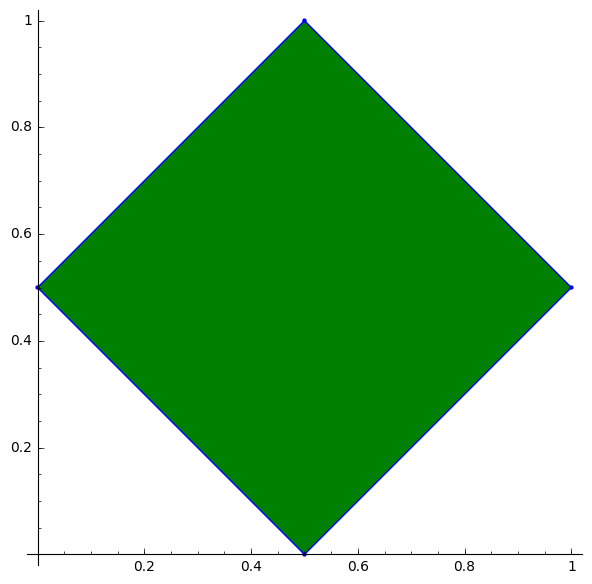
\includegraphics[scale=0.3]{2-dimension-voronoi}
\caption{Voronoi cell in $2$-dimension}
\end{figure}


\begin{figure}[H]
\centering
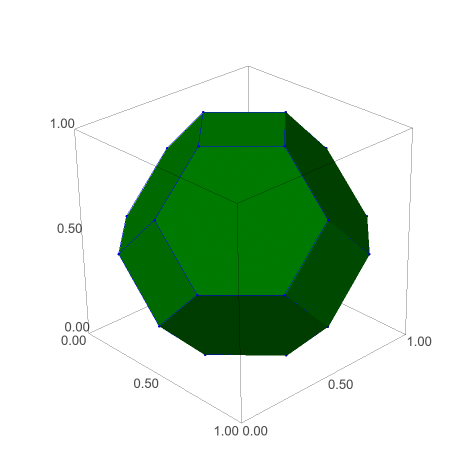
\includegraphics[scale=0.35]{3-dimension-voronoi}
\caption{Voronoi cell in $3$-dimension}
\figuresubtitle{This is not being used in $\mathrm{NewHope}$, only for the purpose of visualization}
\end{figure}


\begin{figure}[H]
\centering
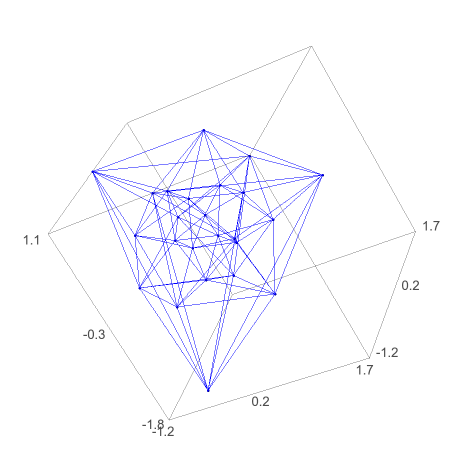
\includegraphics[scale=0.45]{4-dimension-voronoi}
\caption{Voronoi cell in $4$-dimension, (diamond inside a cube)}
\end{figure}


The essence of this new reconciliation can be summarized as the following:
\begin{enumerate}
    \item Divide every coefficient of calculated key, that is: $s' \times (As + e)$ or $s \times (As' + e')$ by $q$. Therefore we a get a list of numbers that are between $[0,1)$ inclusive
    \item Pairwise select every $4$ coefficient $(c_{i}, c_{i+1}, c_{i+2}, c_{i+3})$ and run the $p_{i} = \mathrm{CVP}_{4}(c_{i}, c_{i+1}, c_{i+2}, c_{i+3})$ to get the closest center of Voronoi cell, then store the result into array $[p_{1}, \dots, p_{\frac{n}{4}}]$
    \item For all $p_{i}$ in the array, calculate the distance between $(c_{i}, c_{i+1}, c_{i+2}, c_{i+3})$ and $p_{i}$ and store the result into another array $[d_{i}, \dots, d_{\frac{n}{4}}]$
    \item Send the array $[d_{i}, \dots, d_{\frac{n}{4}}]$ to other party. Note that similar to Ding and Peikert's method, only one party sends the reconciliation information
    \item For all $d_{i}$ in the array, both parties will then add the $d_{i}$ to their $(c_{i}, c_{i+1}, c_{i+2}, c_{i+3})$, so vectors constructed by coefficients of both parties will gets closer to center of closest Voronoi cell. As a result, we will achieve \textit{exact} key agreement
    \item If an adjusted vector generated by $4$ coefficients is in center Voronoi cell then bit is $1$; else bit is $0$
\end{enumerate}



\begin{figure}[H]
    \centering
    \begin{tikzpicture}[scale=1.7]
        \draw[->] (-1,0)--(2,0) node[right]{$x$};
        \draw[->] (0,-1)--(0,2) node[above]{$y$};
        
        \draw[thick] (0, 0.5) -- (0.5,0);
        \draw[thick]  (0.5,0) -- (1,0.5);
        \draw[thick]  (0,0.5) -- (0.5,1);
        \draw[thick]  (0.5,1) -- (1,0.5);
        
        \draw[thick,|<->|] (0,-0.5) -- (1,-0.5);
        \draw[thick,|<->|]  (-0.5,0) -- (-0.5,1);
        
         \fill (0.5,0.5)  circle[radius=1.5pt];
         \fill (0,0)  circle[radius=1.5pt] node[very thick, below left]{$(0,0)$};
         \fill (1,0)  circle[radius=1.5pt] node[very thick, below right]{$(1,0)$};
         \fill (0,1)  circle[radius=1.5pt] node[very thick, above left]{$(0,1)$};
         \fill (1,1)  circle[radius=1.5pt] node[very thick, above right]{$(1,1)$};
        
        \draw[thick,<-]  (0.6,0.5) -- (2,0.5) node[very thick, right]{$(\frac{1}{2},\frac{1}{2})$};
        
        \draw[dotted] (0.5,1) -- (0,1.5);
        \draw[dotted] (0,0.5) -- (-0.5,1);
        \draw[dotted] (-0.5,1) -- (0,1.5);
        
        \draw[dotted] (1.5,1) -- (1,1.5);
        \draw[dotted] (1.5,1) -- (1,0.5);
        \draw[dotted] (0.5,1) -- (1,1.5);
        
        \draw[dotted] (1,0.5) -- (1.5,0);
        \draw[dotted] (0.5,0) -- (1,-0.5);
        \draw[dotted] (1.5,0) -- (1,-0.5);
        
        \draw[dotted] (0,0.5) -- (-0.5,0);
        \draw[dotted] (0.5,0) -- (0,-0.5);
        \draw[dotted] (-0.5,0) -- (0,-0.5);

   \end{tikzpicture}
    \caption{$2$-dimension Voronoi cell centered at $(\frac{1}{2}, \frac{1}{2})$}
\end{figure}

\begin{plain}
\normalfont
The valid Voronoi cell (or Polyhedron generated by Diamond cutting algorithm) should have a volume (or area in $2$-dimensions) of $\frac{1}{2}$ \cite{481786}.
\end{plain}
Above implies that probability of $0, 1$ bits are both equal to $\frac{1}{2}$ in reconciled shared key. Since probability of vector to be inside or outside main Voronoi cell are equal, hence, there is no bias in generated key and it is uniformly distributed.

Below is a simple yet efficient procedure to check if vector generated by coefficients is in main Voronoi cell or otherwise. Subsequently, procedure finds the distance between coefficient vector and center of closest Voronoi cell. The procedure below is for $2$-dimensions, however, for $4$-dimensions it would be similar but $24$ inequalities to check instead of $4$ inequalities. To extract a key from a vector generated by coefficients, it would be similar but returning $1$ if vector is in main Voronoi cell and $0$ otherwise.



\begin{figure}[H]
\centering
% \begin{verbnobox}[\scriptsize]
%             if  (2.0, 2.0) · v - 1.0 >= 0    and (2.0, -2.0) · v + 1.0 >= 0  and
%                 (-1.0, -1.0) · v + 1.5 >= 0  and (-2.0, 2.0) · v + 1.0 >= 0)
        
%                 return (0.5, 0.5) - v
%             else
%                 return round(v) - v
% \end{verbnobox}


\begin{algorithm}[H]
    \caption{get\_distance\_voronoi\_cell}
    \begin{algorithmic}[1]
    \Procedure{get\_distance\_voronoi\_cell}{\textbf{v}}
        \State{\textbf{if} $(2.0, 2.0) \cdot \textbf{v} - 1.0 \ge 0$}
            \State \hspace{\algorithmicindent} $\text{ and } (2.0, -2.0) \cdot \textbf{v} + 1.0 \ge 0$
            \State \hspace{\algorithmicindent} $\text{ and } (-1.0, -1.0) \cdot \textbf{v} + 1.5 \ge 0$ 
            \State \hspace{\algorithmicindent} $\text{ and } (-2.0, 2.0) \cdot \textbf{v} + 1.0 \ge 0$
            \State \hspace{\algorithmicindent} \hspace{\algorithmicindent} \Return $(0.5, 0.5) - \textbf{v}$
        \State{\textbf{else}}
            \State \hspace{\algorithmicindent} \hspace{\algorithmicindent} \Return \texttt{round}(\textbf{v}) - \textbf{v}
    \EndProcedure
    \end{algorithmic}
    \end{algorithm}

    \caption{Finding distance between vector and center of closest Voronoi cell}
    \figuresubtitle{Note that above multiplications with vector \texttt{v} are dot product or scalar product. Also, \texttt{round} function, rounds $x, y$ components of vector \texttt{v} to nearest integer. As $x, y$ are in range $0 \le x, y < 1$ then result of \texttt{round} function would be $ \in \{ (0,0),(0,1),(1,0),(1,1) \}$}
\end{figure}

The idea that one party as a reconciliation information has to send array of (double precision) floating point numbers is not efficient. To resolve the issue Alkim at al. introduced the idea of splitting each Voronoi cells into \iftoggle{verylong}{$2^{rd}=$}{}$16$ sub-cells. Then instead of calculating the distance between vector generated by coefficients and center of closest Voronoi cell, we can find the closest center of Voronoi sub-cell (i.e. sub-cell number that coefficient is located at) and send the sub-cell number to other party as a reconciliation information. Then both parties will add the distance between  lattice point and center of sub-cell to the vector generated by their coefficients; hence they shift the vector generated by their coefficients toward center of their Voronoi cell. Therefore, instead of sending array of distances which are (double precision) floating point numbers, we can send the sub-cell numbers instead which are in integers. Note that we send the sub-cell number and not the outer Voronoi cell number to other party. As a result, eavesdropper does not learn anything from reconciliation information.







\begin{figure}[H]
    \centering
    \begin{tikzpicture}[scale=2.7]
    
    \draw[->] (-0.2,0)--(1.2,0) node[right]{$x$};
    \draw[->] (0,-0.2)--(0,1.2) node[above]{$y$};
    
    
    \draw (0, 0.5) -- (0.5,0);
    \draw (0.5,0) -- (1,0.5);
    \draw (0,0.5) -- (0.5,1);
    \draw (0.5,1) -- (1,0.5);
    
    \draw (0.25,0.75) -- (0.75,0.25);
    \draw (0.375,0.875) -- (0.875,0.375);
    \draw (0.125,0.625) -- (0.625,0.125);
    
    \draw (0.125,0.375) -- (0.625,0.875);
    \draw (0.375,0.125) -- (0.875,0.625);
    \draw (0.250,0.250) -- (0.750,0.750);
    
    \fill (0.5,0.5)  circle[radius=1pt];
    \draw[thick,<-]  (0.6,0.5) -- (2,0.5) node[very thick, right]{$(\frac{1}{2},\frac{1}{2})$};
    

	\fill (0.5,0.875)  circle[radius=0.3pt];
	\fill (0.5,0.625)  circle[radius=0.3pt];
	\fill (0.625,0.5)  circle[radius=0.1pt];
	\fill (0.5,0.375)  circle[radius=0.3pt];
	\fill (0.5,0.125)  circle[radius=0.3pt];


	\fill (0.625,0.750)  circle[radius=0.3pt];
	\fill (0.750,0.625)  circle[radius=0.3pt];
	\fill (0.875,0.500)  circle[radius=0.1pt];

	\fill (0.750,0.375)  circle[radius=0.3pt];
	\fill (0.625,0.250)  circle[radius=0.3pt];
	\fill (0.375,0.250)  circle[radius=0.3pt];
	\fill (0.375,0.500)  circle[radius=0.3pt];
	\fill (0.375,0.750)  circle[radius=0.3pt];

	\fill (0.125,0.500)  circle[radius=0.3pt];
	\fill (0.250,0.625)  circle[radius=0.3pt];
	\fill (0.250,0.375)  circle[radius=0.3pt];

    \end{tikzpicture}
    \caption{$2$-dimension Voronoi cell centered at $ (\frac{1}{2}, \frac{1}{2} )$ split into 16 sub-cells}
\end{figure}

% \subsubsection{Concrete definition of reconciliation}

\iftoggle{long}{
For details on how NewHope reconciliation methods splits Voronoi cell into sub-cells and efficiently finds the sub-cells number in which vector generated by coefficients is located at, translating sub-cell number into Voronoi cell and subsequently extracting a bit form every $4$ coefficients refer to NewHope paper \cite{alkim2015post}.
}{}


\iftoggle{verylong}{
The following is the concrete description of $\mathrm{NewHope}$ reconciliation method. Let $\textbf{B} = (e_1, e_2, e_3, g)$ where $\textbf{g} = (\frac{1}{2}, \frac{1}{2}, \frac{1}{2}, \frac{1}{2})^{T}$ and $e_i$ is the $i$-th vector of unity. Moreover, let $D_4$ be the lattice defined by $\textbf{B}$. The $4$-dimensional space is divided into infinitely many four-dimensional cells, one cell for each lattice vector $\textbf{v}$. In the following we only look at four coordinates of the original vector $\textbf{v}_{R} \in \mathbb{Z}_{q}^{4}$, called $\textbf{v}^{(4)}_{R} \in \mathbb{Z}_{q}^{4}$. The coordinates of $\textbf{v}^{(4)}_{R}$ are divided by $q$ to obtain a vector $x \in \mathbb{R}^{4}/\mathbb{Z}^{4}$. In modulo $\mathbb{Z}^{4}$ there are only two cells in $\mathbb{R}^{4}$, the one corresponding to the lattice vector $\textbf{g}$ and the one corresponding to the lattice vector $(0, 0, 0, 0)^{T}$. If a vector $\textbf{x}$ lies in the cell which belongs to $\textbf{g}$, it is mapped to $1$, otherwise it is mapped to $0$. Determining the correct cell can be done by using algorithm $\mathrm{CVP}_{D_4}$. Since the sender and the receiver do not get exactly the same vectors $\textbf{v}_{S}^{(4)} \approx \textbf{v}_{R}^{(4)}$ that they want to encode in the way described above, they need to be sure that their vectors lie in the same cell. This however is not necessarily true. Hence, they need to exchange some reconciliation information $\textbf{c}^{(4)}$ which defines how the vector $\textbf{v}_{S}^{(4)}$ has to be moved to assure that it is in the same cell as $\textbf{v}_{R}^{(4)}$. For this we divide each cell into $2^{4r}$ sub-cells (if not stated differently, we assume $r = 2$). The receiver assigns the number of the sub-cell of $\textbf{v}_{R}^{(4)}$ to $\textbf{c}^{(4)} \in \{0, 1, 2, 3\}^{4}$ and sends it to the sender. Afterwards, the sender computes the difference vector of the middle of a cell and the middle of the sub-cell corresponding to $\textbf{c}$. Then the sender runs the $\mathrm{CVP}_{D_4}$ algorithm.

If $\textbf{v}_{S}^{(4)} \in \mathbb{Z}^{4}_{q}$ and $\textbf{c}^{(4)} \in \{0, 1, 2, 3\}^{4}$ then

\begin{equation}
\centering
    \mathrm{Rec}(\textbf{v}_{S}^{(4)}, \textbf{c}^{(4)}) = \mathrm{Decode}(\frac{1}{q} \textbf{v}_{S}^{(4)} - \frac{1}{2^r}\textbf{B}\textbf{c}^{(4)})
\end{equation}

computes one bit of the key from four coefficients.

% We identify an element $f(x) \in \mathbb{R}_{q}$ with a vector:
% \[(f_{0}', \dots, f_{\frac{n}{4}}') \in \mathbb{Z}[x] /(x^4 + 1)^{\frac{n}{4}} \text{ such that } f(x) = f'_{0}(x^{\frac{n}{4}}) + x \cdot f'_{1}(x^{\frac{n}{4}}) + \dots + x^{\frac{n}{4}} \cdot f'_{\frac{n}{4}}(x^{\frac{n}{4}})\]


The function $\mathrm{HelpRec}(\textbf{v}_{R})$ in the protocol of the receiver is defined as $\mathrm{HelpRec}(\textbf{v}_{R}^{(4)}) = \mathrm{CVP}_{D_4} (\frac{2^r}{q} (\textbf{v}_{R}^{(4)}) + b  \textbf{g}) \bmod 2^r$, where $b \leftarrow \{0, 1\}$.


\begin{algorithm}[H]
    \caption{CVP$_{D_{4}} (\textbf{x} \in \mathbb{R}^4)$}
    \begin{algorithmic}[1]
        \Procedure{CVP}{\textbf{x}}
            % \State \textbf{Ensure: } an integer vector $z$ such that $B \cdot z$ is closest to vector $x: x-B \cdot z \in \mathscr{V}$
            \State $\textbf{v}_{0} \leftarrow \lfloor \textbf{x} \rceil$
            \State $\textbf{v}_{1} \leftarrow \lfloor \textbf{x} - \textbf{g} \rceil$
            \State $k \leftarrow 0 \texttt{ if } ||\textbf{v} - \textbf{v}_{0}||_{1} < 1 \texttt{ else } 1$
            \State $(\textbf{v}_0, \textbf{v}_1, \textbf{v}_2, \textbf{v}_3)^{t} \leftarrow \textbf{v}_{k}$
            \State \textbf{return:} $(\textbf{v}_0, \textbf{v}_1, \textbf{v}_2, k)^{t} + \textbf{v}_{3} \cdot (-1, -1, -1, 2)^t$
        \EndProcedure
    \end{algorithmic}
\end{algorithm}

\begin{algorithm}[H]
    \caption{Decode $(x \in \mathbb{R}^4 / \mathbb{Z}^4)$}
    \begin{algorithmic}[1]
        \Procedure{Decode}{x}
            % \State \textbf{Ensure: } a bit $k$ such that $k \cdot g$ is closest vector to $x + \mathbb{Z}^4: x - kg \in \mathscr{V} + \mathbb{Z}^4$
            \State $\textbf{v} \leftarrow \textbf{x} - \lfloor \textbf{x} \rceil$
            \State $r \leftarrow  0 \texttt{ if } ||\textbf{v}||_{1} \le 1 \texttt{ else } 1$
            \State \textbf{return:} $r$
        \EndProcedure
    \end{algorithmic}
\end{algorithm}
}

Furthermore, NewHope protocol generates the shared polynomial pseudo-randomly on every run of the KEM to assure safety against backdoors. Next chapter discusses the method as suggest in NewHope protocol to efficiently share the shared polynomial with other party. In essence, to generate a pseudo-random polynomial $A$, NewHope uses a $256$-bit seed and a type of hash-function that outputs arbitrary length, e.g., $\mathrm{SHAKE}$-128. This can be done similarly for all the other protocols.





\subsubsection{Generalized form of randomized doubling function suggested by Alkim et al.}
The probability of $\textbf{x}$ being in a center Voronoi cell is the same as for $\textbf{x}$ being in other Voronoi cells. This would be the case if $\textbf{x}$ actually followed a continuous uniform distribution. However, the coefficients of $\textbf{x}$ are discrete values in $\{0,\frac{1}{q},\dots,\frac{q-1}{q}\}$ and with the protocol described so far, the bits of $\textbf{v}$ would have a small bias. The solution is to add to $\textbf{x}$ with probability $\frac{1}{2}$ the vector $(\frac{1}{2q}, \dots, \frac{1}{2q})$ before running the error reconciliation. This has close to no effect for most values of $\textbf{x}$, but, with probability $\frac{1}{2}$ moves $\textbf{x}$ to another Voronoi cell if it is very close to one side of a border.

In the example below we see that $72$ dots ($36$ red and $36$ black ones) remain in their Voronoi cell; the other $9$ dots ($4$ red and $5$ black ones) change Voronoi cell with probability $\frac{1}{2}$ which precisely eliminates the bias in the key.

\begin{figure}[H]
\centering
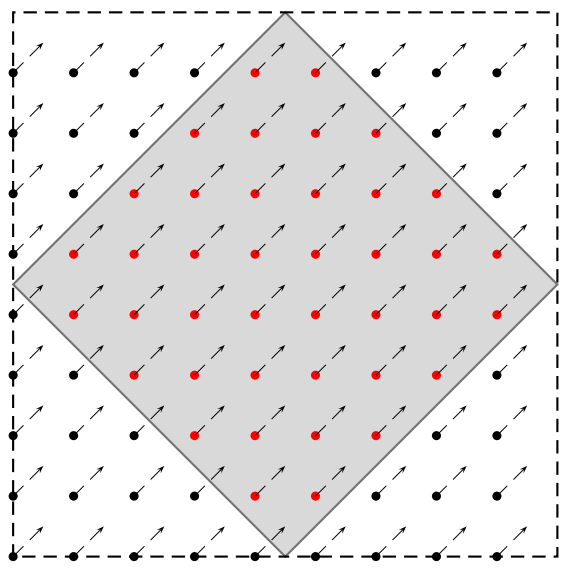
\includegraphics[scale=0.3]{dbl_newhope}
\caption{Effect of generalized form of randomized doubling function on vectors}
\end{figure}







